\documentclass[11pt]{article}
\usepackage[a4paper, left=0.75in, right=0.75in, top=0.5in, bottom=0.5in]{geometry}
\usepackage{amsmath, bm}
\usepackage{amssymb}
\usepackage{solarized-light}
\usepackage{hyperref}
\hypersetup{
    colorlinks=true,
    linkcolor=blue,
    filecolor=magenta,      
    urlcolor=blue,
}
\usepackage{graphicx}
\graphicspath{ {.} }

\title{ES 404 - Assignment 1}
\date{}
\author{Nishant Tatar - 21110223}

\begin{document}
\maketitle

\section{Question 1}
\subsection{Nodes and Links}
The Nodes are the people interacting with each other via tweets and edges are the tweets.\\
Edges for now are of three types: A - A (Author - Author) ; A - R (Author - Retweeter) ; R - R (Retweeter - Retweeter)
\subsection{Size}
The number of nodes in the network: $>400$ \\
The number of Edges in the network: $>3000$ 
\subsection{Mapping}
Yes, the Network can be mapped out.
\subsection{Importance}
The analysis of this network can provide key insights into how fake news can spread, the major pathways that it uses, and how it can be curtailed in this era of disinformation.

\subsection{Citation}
This particular question of the Assignment has been discussed with Hitesh Jaiswal, as he is my project partner and we are working in the same group, the rest of the assignment is my own and I have not discussed with anyone.


\section{Question 2}
\textbf{Prework}: \\
Given an N x N matrix $\mathbf{A}$, an $\mathbf{1}$ as the column vector, the following can be said:

\subsection{Degree Vector $k$ :}

The degree vector $k$ can be written as $A \cdot 1 = k$, as $k_i$ will be a result of the summations of the entries in the rows of $A$ and the singular column of $1$.

\subsection{Total Links in the Network:}

Since $A_{ij}$ of the adjacency matrix $A$ represents the connection between two particular nodes, the diagonal entries will be $0$ as it has no self loops, we can write that half the sum of the matrix will be the number of Links in the network. Since it is a weighted Network, I am assuming that the weight of each link is classified as a single link counted that many number of times. Such that for a weight of 2, it is 2 links between those particular nodes.
\\ \\
Hence, the total number of links in the network can be represented by:
\begin{equation}
    L = \frac{1^T A 1}{2}
\end{equation}

\subsection{Number of Triangles:}
$A_{ij}^k$ represents the number of k step paths from node i to j. Using the same, starting at i and ending at i for a closed triangle, the entires at $A_{ii}^3$ will represent the information required. The total number of triangles can be obtained by $\text{Tr}(A^3)$. However, Since this is an undirected network, each triangle is counted clockwise as well as counter-clockwise and the triangle will be counted for each node, therefore the actual number of triangles can be calculated using:
\begin{equation}
    N_T = \frac{\text{Tr}(A^3)}{6}
\end{equation}

\subsection{Degree Vector for Neighbor Degree Nodes:}

The degree vector $k$ signifies the degree of each node. Using $k\cdot A$, the resultant due to matrix multiplication will be the sum of the degrees of the neighbors of the node $k_i$. Hence the Vector required can be obtained using $ k \cdot A$.

\subsection{Degree Vector for Second Neighbor Degree Nodes:}

Here, we can think of this as follows. $A^3$ represents the number of unique 3 step paths. $A^3 \cdot k$  gives the second degree sum. However, this also does count the first degree neighbors and does not discard loops either. So we need to take care of that also. 
\\
The subtraction term maybe written as follows: $(A\cdot1)^2$, where each term in the returned vector is squared.
\\
Therefore, the Vector that signifies the sum of second neighbors of a node in a network can be written by: $A^3 \cdot k - (A\cdot1)^2$ \\
\\
\textbf{Sample Network of 4x4}: \\ \\
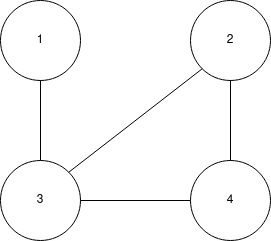
\includegraphics[scale=0.5]{graph.png}
\\
\noindent The Adjacency Matrix $A$ of this network will be: 
$ \begin{bmatrix}
    0 & 0 & 1 & 0 \\
    0 & 0 & 1 & 1 \\
    1 & 1 & 0 & 1 \\
    0 & 1 & 1 & 0

\end{bmatrix}$

\subsection{Sample Matrix Degree Vector K}
$ A \cdot 1 = k$ \\ \\ 
$ \begin{bmatrix}
    0 & 0 & 1 & 0 \\
    0 & 0 & 1 & 1 \\
    1 & 1 & 0 & 1 \\
    0 & 1 & 1 & 0
\end{bmatrix}
\times
\begin{bmatrix}
    1 \\
    1 \\
    1 \\
    1 
\end{bmatrix}
=
\begin{bmatrix}
    1 & 2 & 3 & 2
\end{bmatrix}$

\subsection{Sample Matrix Total Links}
$L = \frac{1^T A 1}{2}$ 
\\
$\therefore L = 8/2 = 4$
\\
Which is the number of links in the network.

\subsection{Number of Triangles in sample network:}

$N_T = \frac{\text{Tr}(A^3)}{6}$
\\
For the Adjacency Matrix A: $ \begin{bmatrix}
    0 & 0 & 1 & 0 \\
    0 & 0 & 1 & 1 \\
    1 & 1 & 0 & 1 \\
    0 & 1 & 1 & 0

\end{bmatrix}$ , $A^3$ will be: $ \begin{bmatrix}
    0 & 1 & 3 & 1 \\
    1 & 2 & 4 & 3 \\
    3 & 4 & 2 & 4 \\
    1 & 3 & 4 & 2
\end{bmatrix}$ \\
$\text{Tr}(A^3)$ = 6.
Therefore the total number of Triangles is 1.

\subsection{Degree Vector for neighboring Nodes:}
$k \cdot A$ \\
$ \begin{bmatrix}
    1 & 2 & 3 & 2
\end{bmatrix}
\times
\begin{bmatrix}
    0 & 0 & 1 & 0 \\
    0 & 0 & 1 & 1 \\
    1 & 1 & 0 & 1 \\
    0 & 1 & 1 & 0
\end{bmatrix}
=
\begin{bmatrix}
    3 & 5 & 5 & 5
\end{bmatrix}
$

\subsection[short]{Degree Vector for second neighbors:}

$A^3 \cdot k - (A\cdot1)^2$ \\

$
\begin{bmatrix}
5 \\
10 \\
13 \\
10
\end{bmatrix}
-
\begin{bmatrix}
    1 \\
    4 \\
    9 \\ 
    4
\end{bmatrix}
=
\begin{bmatrix}
    4\\
    6\\
    4\\
    6
\end{bmatrix}
$

\section{Question 3}
Code used for this:\\ 
Colab Link: \href{https://colab.research.google.com/drive/1ZiCxfnfzeQLUYKbacRC6YViKvvSxXons?usp=sharing}{Link to Notebook} \\

\subsection{Network Generation}

For Subcritical Regimes, the probability required is in the range of $p < \frac{1}{N-1}$. As such, the probability for network generation is taken as $\frac{1}{2 (N-1)}$ \\
For Critical Regimes, the probablity is $p = \frac{1}{N-1}$. \\
For Supercritical Regimes, the probability required is in the range of $ \log(N) > p > \frac{1}{N-1}$ and is taken as $\frac{2}{(N-1)}$ 

\subsection{Visualisation}
Subcritical Regime:\\
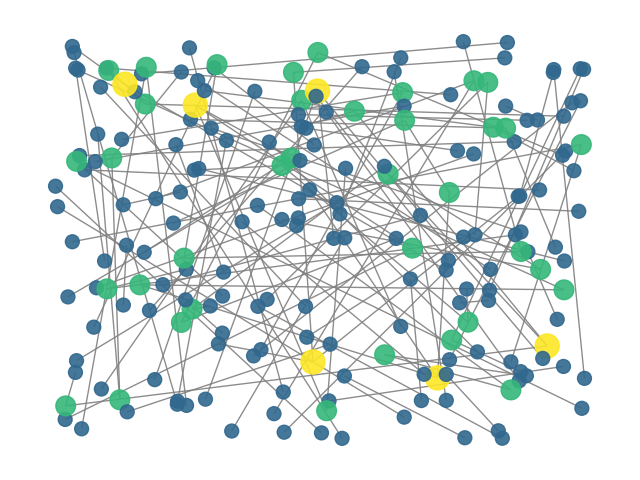
\includegraphics[scale=0.5]{subcgv.png} \\ 
Critical Regime: \\
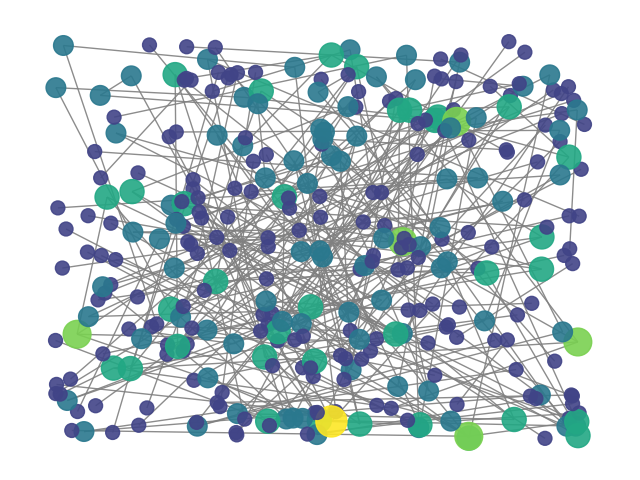
\includegraphics[scale=0.5]{cgv.png} \\ 
SuperCritical Regime:\\
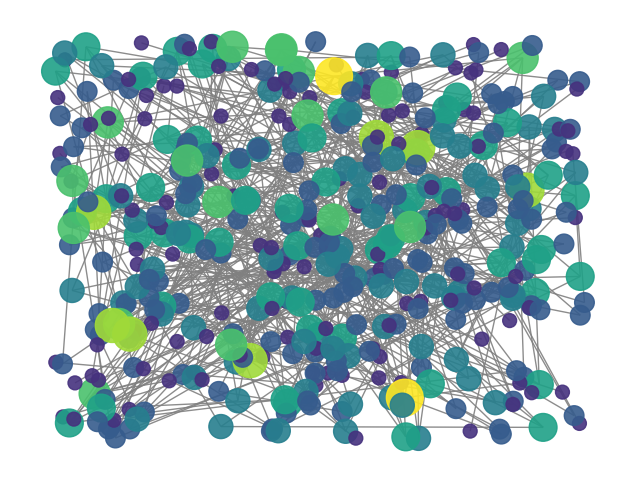
\includegraphics[scale=0.5]{supcgv.png}

\subsection{Degree Distribution Plotting}

Subcritical Regime:

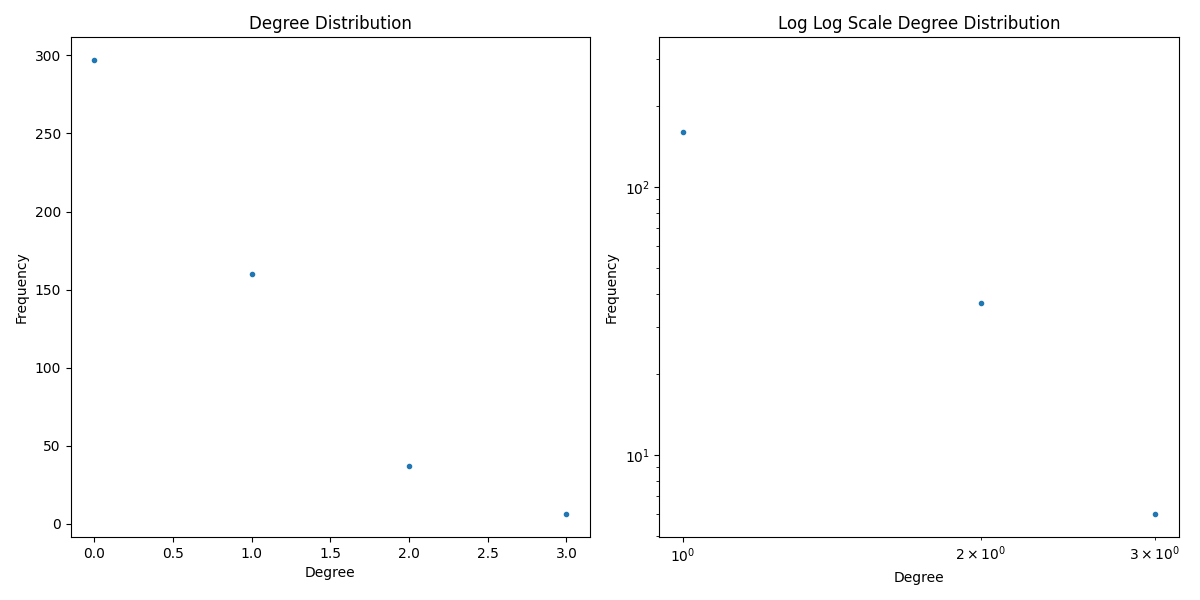
\includegraphics[scale=0.5]{subcgdis.png}

Critical Regime:

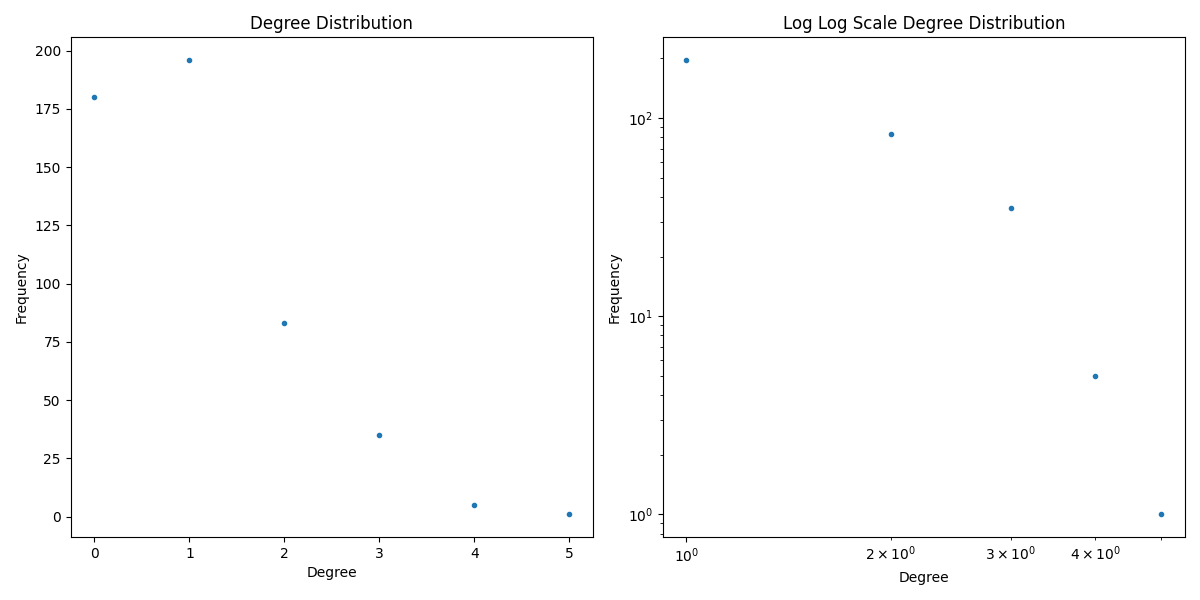
\includegraphics[scale=0.5]{cgdis.png}

SuperCritical Regime:

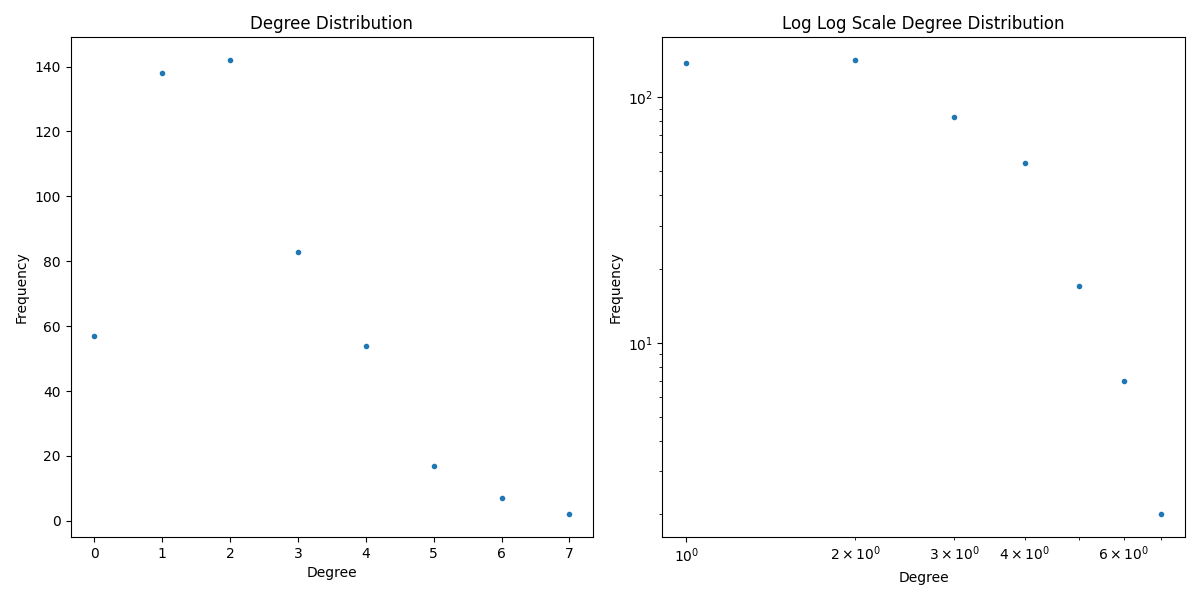
\includegraphics[scale=0.5]{supcgdis.png} \\
In the Subcritical regime, an extreme number of nodes have no degree, and are not connected to each other, and as such, the network is very sparse and has very low connectivity. \\ \\
Contrasted with the critical regime, the number of nodes which have at least 1 degree is increased, and as such the network is more connected. However, there is still a major fraction of nodes which are unconnected.\\ \\
In the SuperCritical Regime, the number of nodes that are not part connected to another node falls sharply, and the network starts to approach the fully conected regime.

\subsection{Statistical Analysis}

For Conducting the P Value test, I generated a poisson distribution. Using KS test to compare between network degree distribution and poisson distribution, we get the p value.\\ 
We set the Hypothesis to be that the distribution follows the poisson process. In all three cases, the P value is very close to 1, to the extent that we can very reasonably call these poisson distributions. \\

\subsection{Largest Connected Cluster Analysis}

Subcritical: \\
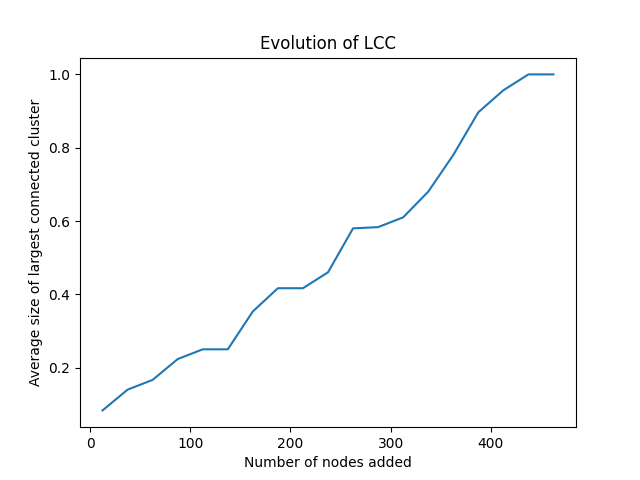
\includegraphics[scale=0.5]{nevol.png}

Critical:\\
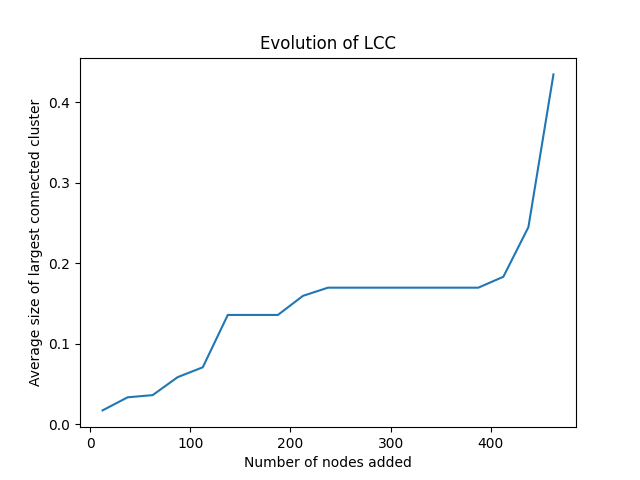
\includegraphics[scale=0.5]{nevolc.png}

Supercritical:\\
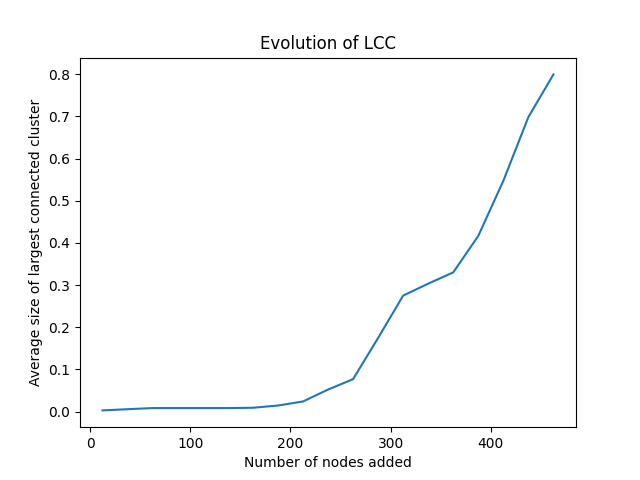
\includegraphics[scale=0.5]{nevolsupc.png}

From the Graphs, the subcritical regime is the most reistant to change, which also makes sense, since the size of the LCC is very low, the probable effect of removing a node from the network is very low as compared to the supercritical regime, where the size of the LCC is higher, and the number of nodes not part of the LCC much lower. However, in terms of network connectivity, the supercritical regime is much better, as the number of nodes that are in the LCC is much higher, and new nodes coming to the network have higher chance of joining the LCC.

\section{Question 4}
Code used for this:\\ 
Colab Link: \href{https://colab.research.google.com/drive/1IO6M2aksI1LgTy-kVjHkXarPsqFt2RmS?usp=sharing}{Link to Notebook} \\

\subsection{Network Generation}
For Anamalous Regimes, $\gamma < 2$ therefore, taking $\gamma = 1.9$ \\ 
For Scalefree Regimes, $3 > \gamma > 2$ therefore, taking $\gamma = 2.6$ \\ 
For Anamalous Regimes, $\gamma > 3$ therefore, taking $\gamma = 3.8$ 
\subsection{Visualisation}
Anamalous: \\
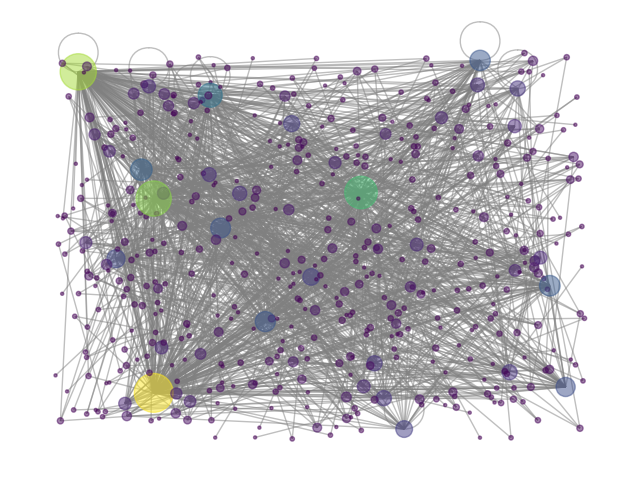
\includegraphics[scale=0.5]{gvanam.png}

Scale-Free: \\
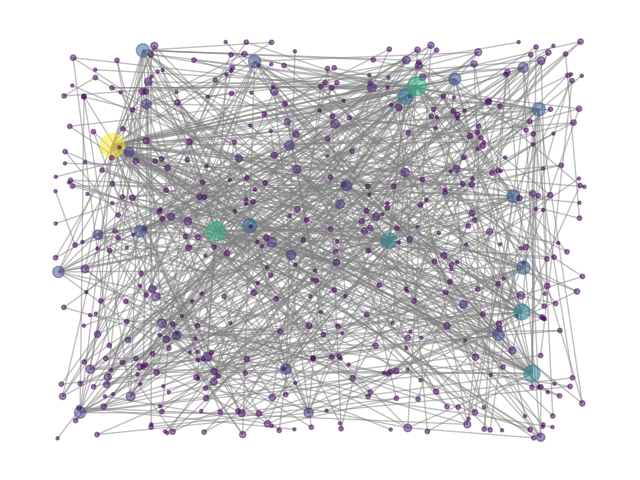
\includegraphics[scale=0.5]{gvsf.png}

Random Regime: \\
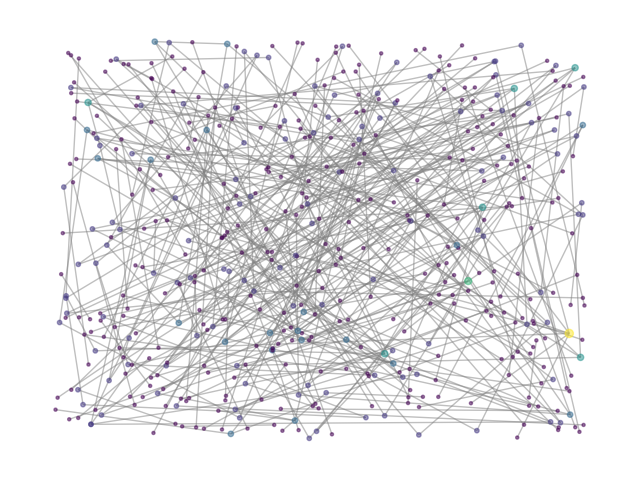
\includegraphics[scale=0.5]{gvrand.png}

\subsection{Degree Distribution Plotting}
Anamalous: \\
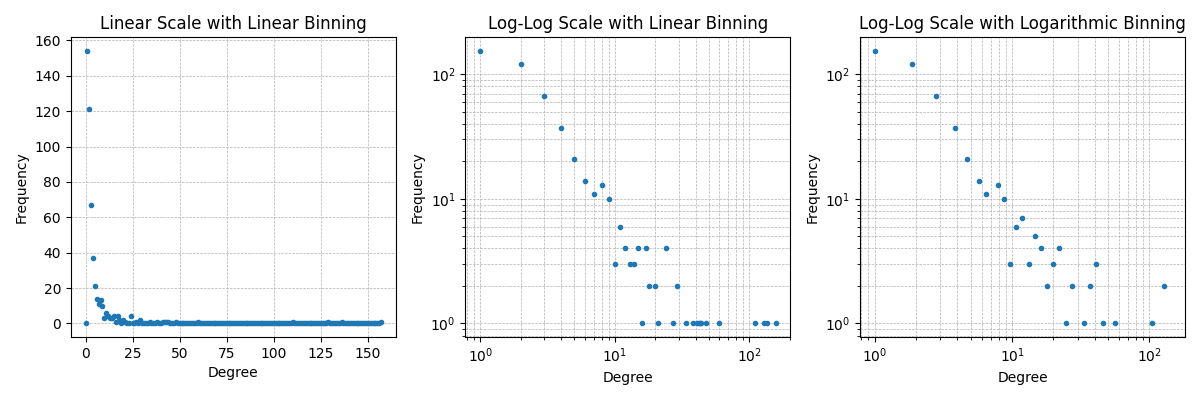
\includegraphics[scale=0.5]{dganam.png}

Scale-Free: \\
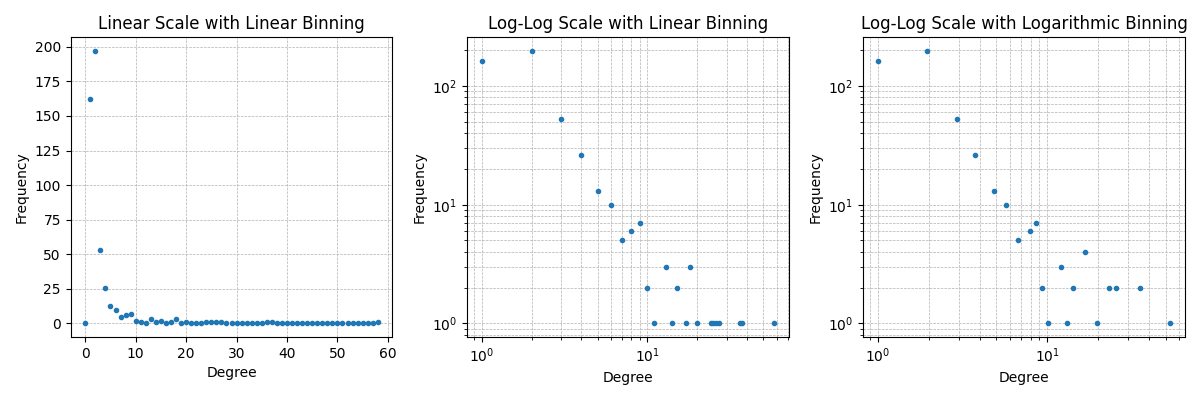
\includegraphics[scale=0.5]{dgsf.png}

Random Regime: \\
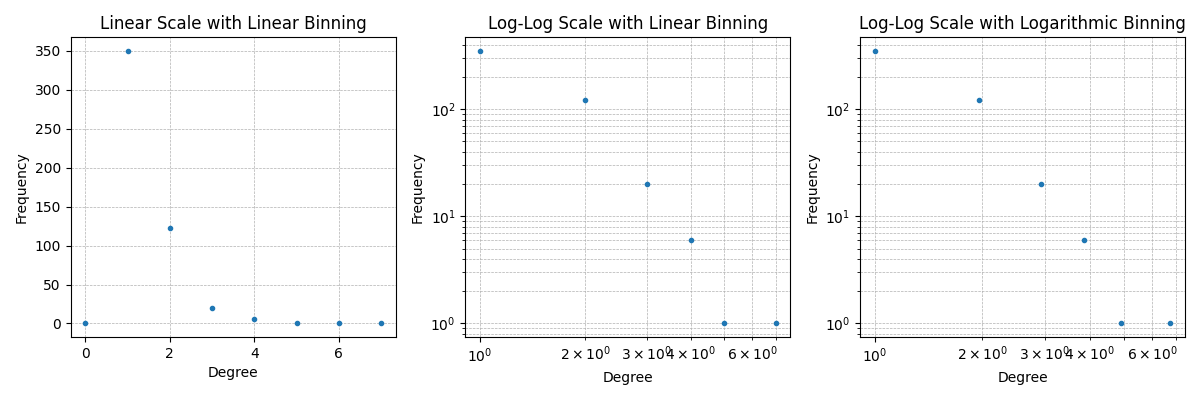
\includegraphics[scale=0.5]{dgrand.png}
\\
When $\gamma < 2$, it is an anamalous regime, where the network is distributed as maximum number of nodes having only a single degree, while there is a steady presence of nodes as the degree of interest of nodes is increased.
\\
When $3 > \gamma > 2$, the network lies in the scalefree regime, where a few hubs connect to a large number of nodes that have a single degree.
\\
When $\gamma > 3$, the network starts to behave like a random network. It is not a random network, but it starts exhibiting many of the properties of random network.

\subsection{Statistical Analysis}

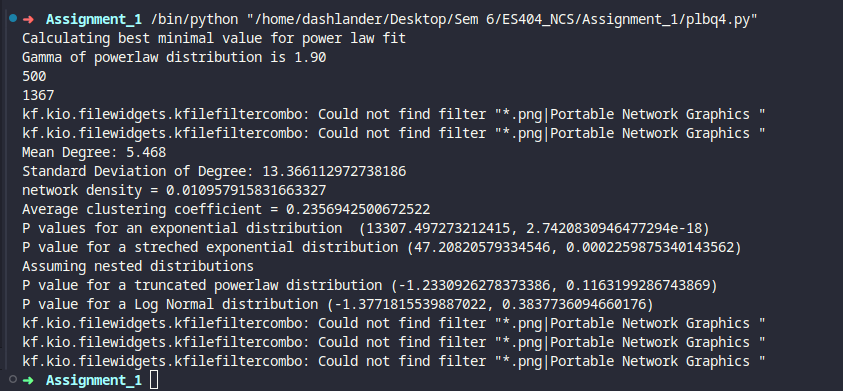
\includegraphics[scale=0.7]{statsanam.png}\\
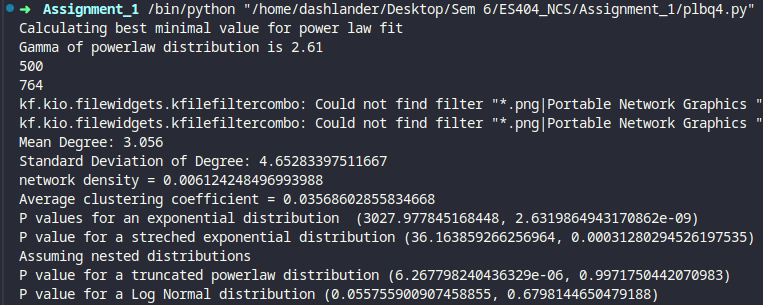
\includegraphics[scale=0.7]{statssf.png}\\
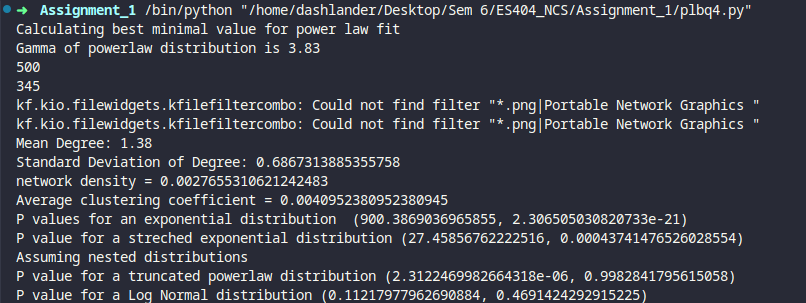
\includegraphics[scale=0.7]{statsrand.png}\\
The Network in the Anomalous regime has a higher mean degree as well as a standard deviation that goes higher. This is due to the fact that both are unbounded in this region. Compartively, in the Scalefree regime, the Mean is lower, as is the standard deviation. In the random regime, most nodes will have nearly the same number of degree, with the probability of hubs arising being very low.\\ \\
Using the distribution compare function from the powerlaw package, we find the P values of the distribution with that of standard distributions.\\ \\
From the given data, we see that for the Anomalous regime, the Log Normal distribution has the highest P value, for the scalefree and random regimes the Powerlaw distribution has the highest P values. As such, in the scalefree regime, it is a powerlaw distribution.

\subsection{Network Analysis: Local Clustering Coefficient}
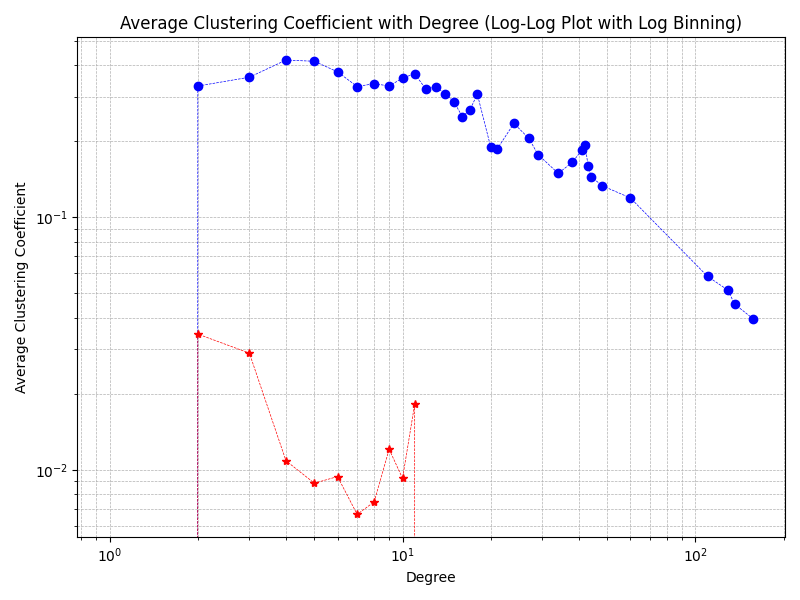
\includegraphics[scale=0.5]{ccanam.png}\\
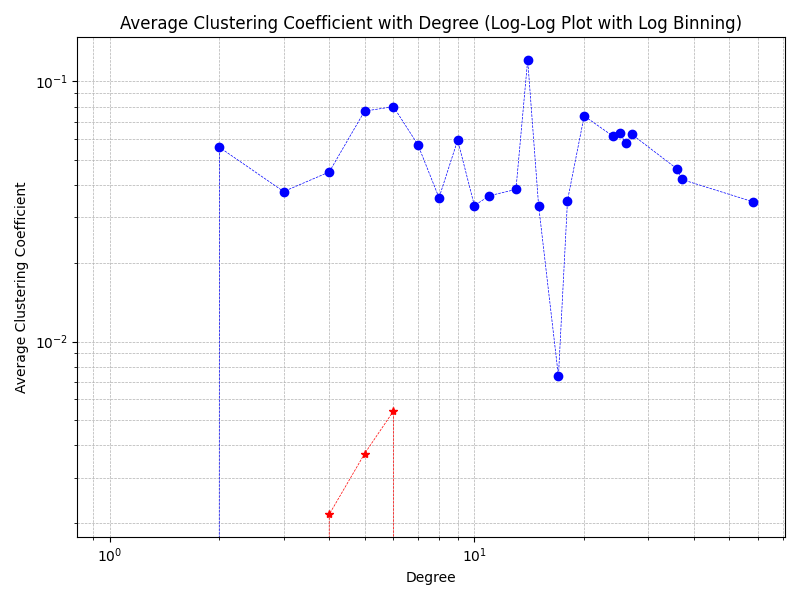
\includegraphics[scale=0.5]{ccsf.png}\\
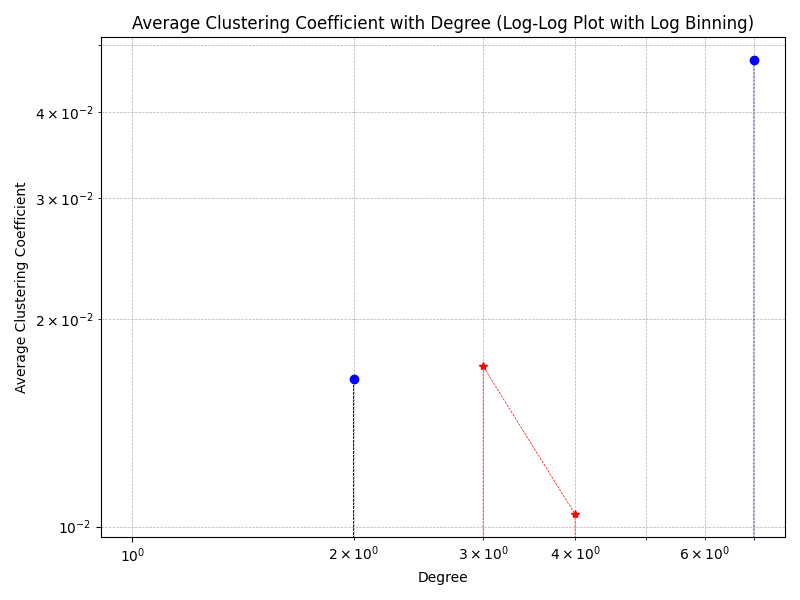
\includegraphics[scale=0.5]{ccrand.png}\\
The Clustering Coefficient for a network in the Anomalous regime will be higher, as there are more nodes whose neighbors are higher degree nodes as compared to those in Scalefree or Random regimes, which can also be seen from the fact that the graphs for scalefree and random regimes are much less distinct in log log scales.\\
The red line denotes the expected Clustering Coefficients from an ER network that has the same number of nodes and links. As can be observed, the ER network does not have nodes with higher degrees.

\subsection{Network Resilience}
Anomalous Regime:\\
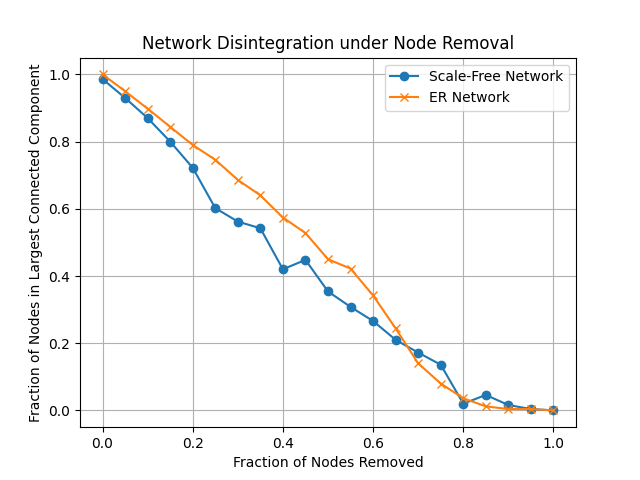
\includegraphics[scale=0.5]{rnranam.png} 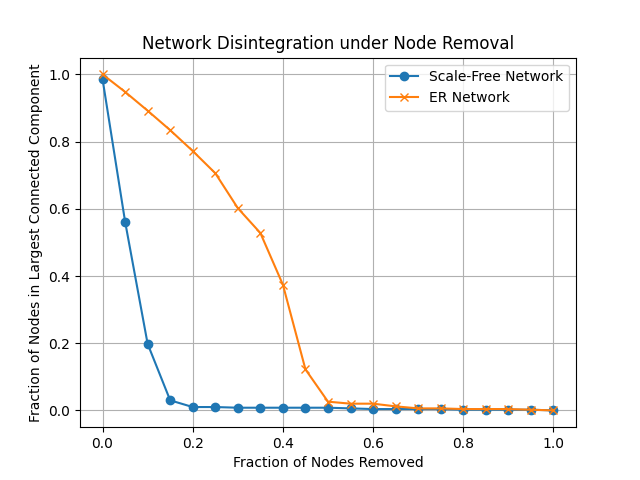
\includegraphics[scale=0.5]{tnranam.png}\\
Scalefree Regime:\\
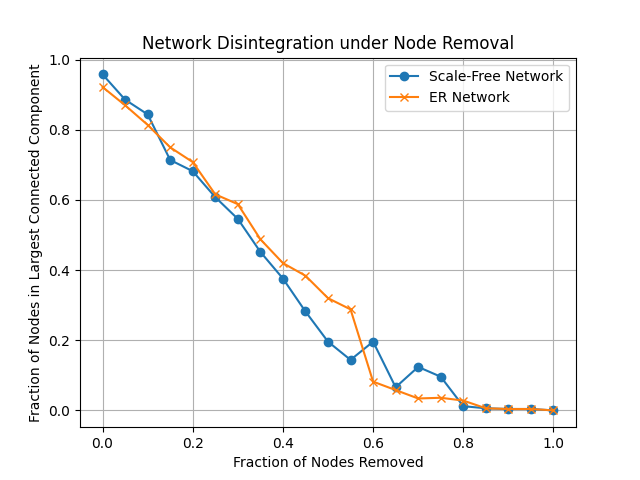
\includegraphics[scale=0.5]{rnrsf.png} 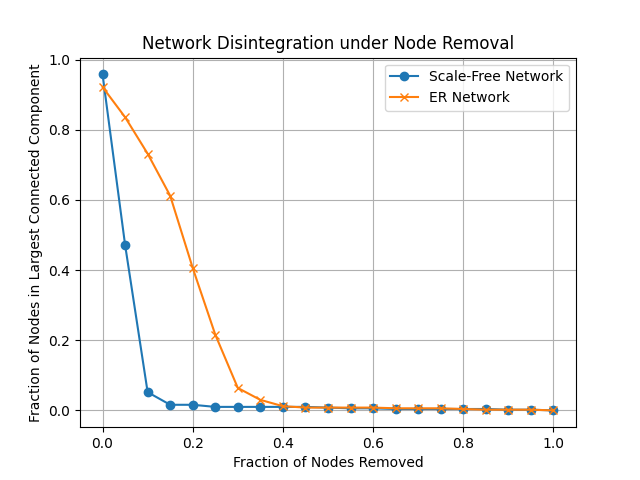
\includegraphics[scale=0.5]{tnrsf.png}\\
Random Regime:\\
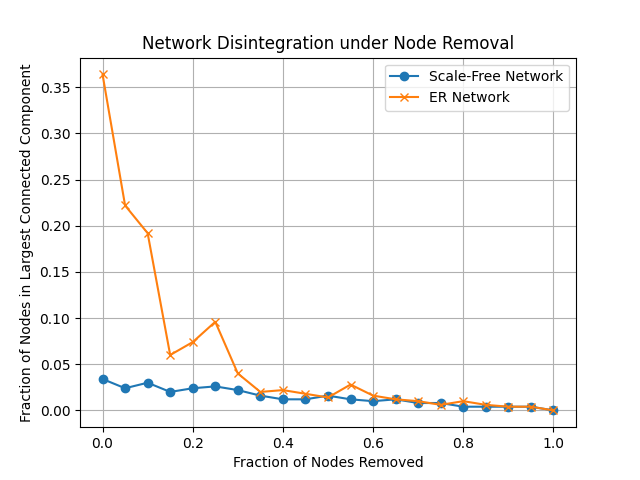
\includegraphics[scale=0.5]{rnrrand.png} 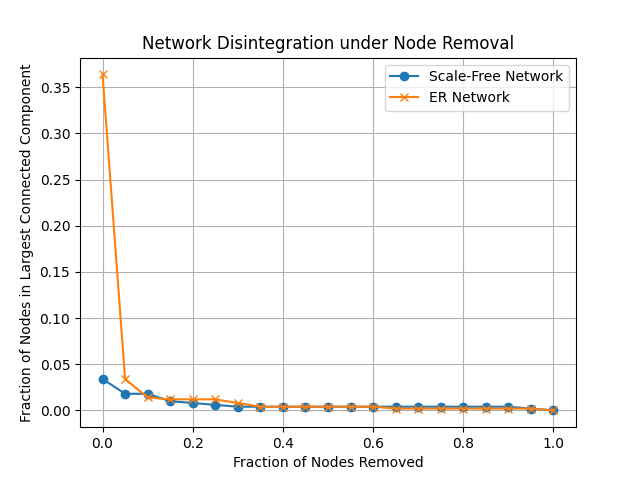
\includegraphics[scale=0.5]{tnrrand.png}\\
As can be seen, in both random and targetted removal of nodes, the ER network is much more resilient compared to it's equivalent powerlaw network in both scalefree and random regimes, as the powerlaw network has the presence of hubs, which are not present in the ER network.\\
As such, the ER network requires more fraction of nodes to be removed as compared to the powerlaw network for the fraction of it's nodes in the Largest Connected Cluster to drop down significantly. This is seen much more starkly in targetted removal of nodes, where the nodes with the highest degree is removed.

\section{Question 5}
\subsection{Average Degree Calculation}
Focusing on Blue nodes(as they can be treated as equivalent, and results will be similar), the average degree of the subnetwork with blue nodes will be: $\langle k_b \rangle = p(N-1)$ . The same can be said for the average degree of the subnetwork with red nodes: $\langle k_r \rangle = p(N-1)$.\\ \\
When considering the average degree for nodes when both types of nodes are considered, blue nodes will connect to $N-1$ blue nodes with probability $p$ and $N$ nodes with probability $q$. The average degree of blue nodes will be $\langle k_b \rangle = p(N-1) + qN$ . Red nodes will connect to $N-1$ red nodes and $N$ blue nodes, and as such the average degree will be $\langle k_r \rangle = p(N-1) + qN$.\\
The average degree will be:\\
$$\langle k_{avg} \rangle = \frac{\langle k_b \rangle + \langle k_r \rangle}{2}$$

\subsection{Network Connectivity}
As this is a random graph, using the ER concept of full network connectivity at $ p > \frac{\ln{N}}{N}$, we can say that for the network to be connected at least for the two subnetworks, we know the mimimum p value for the network.\\
A single edge between a red and blue node will ensure that the network is fully connected, as the blue and red subnetworks are fully connected setting the value of p as greater than $\frac{\ln{N}}{N}$. As a node can connect to $N$ nodes of opposite color, the minimum value of q is $\frac{1}{N}$ for one node. However, there are N nodes, as such, there the minimum value of q will be $\frac{1}{N^2}$.\\
Therefore, the minimum values of p and q for a fully connected network are:\\
$$ p > \frac{\ln{N}}{N} $$
$$ q > \frac{1}{N^2} $$
As the network grows, p will increase, to ensure connectivity for the subnetworks, and q can decrease to the extent that at least one connection exists between the red and blue subnetworks.

\subsection{Snobbish Networks}
Assuming that $ p >> q $, we can still say that it exhibits small world property. We can say that this is true, because the maximum network path length between two nodes will be between Blue and Red nodes, and even then if we assume that there is only one connection between Red and Blue nodes, if the network distance is $d$, the network distance will become $2d + 1$ in the extreme case. Where the network distance $d$ is given by $\ln{N}$, this is still a very small value when compared to N. As such, we can reasonably say that even Snobbish networks will exhibit small world properties.\\
A sample Python code that showcases this is given here: \href{https://colab.research.google.com/drive/1WSJCAuKiGnRM3uf4ftNwsbB8xiSTxdVr?usp=sharing}{Link to Notebook}

\end{document}